\documentclass{aip-cp}

\usepackage[numbers]{natbib}
\usepackage{rotating}
\usepackage{graphicx}
\usepackage{enumitem}
\pdfmapfile{+txfonts.map}

%%%%%ДОБАВИЛ ДЛЯ РУССКОГО ТЕКСТА
\usepackage[utf8x]{inputenc}
\usepackage[english,russian]{babel}
\usepackage{cmap}
%%%%%


% Document starts
\begin{document}

% Title portion
\title{The Title Goes Here with Each Initial Letter Capitalized}

\author{Victor Gergel\corref{cor1}}
\author{Konstantin Barkalov}
%\eaddress[url]{http://www.aip.org}
\author{Ilya Lebedev}
%\eaddress{anotherauthor@thisaddress.yyy}
\author{Maria Rachinskaya}

\affil{Lobachevsky State University of Nizhni Novgorod, Nizhni Novgorod, Russia.}
\corresp[cor1]{Corresponding author: gergel@unn.ru}

\maketitle

\begin{abstract}
В работе рассматривается дальнейшее развитие подхода к построению тестовых задач глобальной оптимизации с нелинейными ограничениями. Для порождаемых задач расположение глобального минимума является известным.
Отличительной чертой рассматриваемого генератора является возможность указания желаемого количества ограничений и доли допустимой области относительно все области глобального поиска. В обновленной версии генератора добавлена возможность формирования задач с условным минимумом, расположенным на границе допустимой области, и указания числа ограничений, активных в точке минимума. Демонстрация разработанного подхода приводится на примере известного индексного метода для решения сложных многоэкстремальных задач оптимизации с нелинейными ограничениями.
\end{abstract}

% Head 1
\section{INTRODUCTION}

In the present paper, the methods for generating the global optimization test problems with non-convex constraints
\begin{eqnarray}
&\varphi(y^\ast)=\min{\left\{\varphi(y):y\in D, \; g_i(y)\leq 0, \; 1 \leq i \leq m\right\}}, \label{i_problem} \\
&D=\left\{y\in R^N: a_i\leq y_i \leq b_i, 1\leq i \leq N\right\} \label{D}
\end{eqnarray}
are considered. The objective function $\varphi(y)$ (henceforth denoted by $g_{m+1}(y)$) and the left-hand sides $g_i(y), \; 1\leq i \leq m,$ of the constraints are supposed to satisfy the Lipschitz condition
\[ \left|g_i(y')-g_i (y'')\right| \leq L_i \left\|y'-y'' \right\|, \; y',y''\in D, \; 1\leq i \leq m+1. \]
with the Lipschitz constants unknown a priori. The analytical formulae of the problem functions may be unknown, i.e. these ones may be defined by an algorithm for computing the function values in the search domain (so called ``black-box''-functions). It is supposed that even a single computing of a problem function value may be a time-consuming operation since it is related to the necessity of numerical modeling in the applied problems (see, for example, \cite{Menniti2008,Kvasov2015,Modorskii2017}).

The evaluation of efficiency of the developed methods is one of the key problems in the optimization theory and applications. Unfortunately, it is difficult to obtain any theoretical estimates in many cases. As a result, the comparison of the methods is performed by carrying out the computational experiments on solving some test optimization problems in most cases. In order to obtain a reliable evaluation of the efficiency of the methods, the sets of test problems should be diverse and representative enough. The problem of choice of the test problems has been considered in a lot of works (see, for example, \cite{Floudas1999,Gaviano2003,Ali2005,Addis2007}). Unfortunately, in many cases, the proposed sets contain a small number of test problems, and it is difficult to obtain the problems with desired properties. The most important drawback consists of the fact that the constraints are absent in the proposed test problems as a rule (or the constraints are relatively simple: linear, convex, etc.).

В данной работе проводится дальнейшее развитие подхода для порождения задач глобальной оптимизации с нелинейными ограничениями, первоначально предложенного в \cite{Gergel2017}. При генерации тестовых задач может быть указано необходимое количество ограничений и желаемая доля допустимой области относительно все области глобального поиска. При этом для порождаемых задач расположение глобального минимума является известным, что существенно упрощает оценку результатов выполненных вычислительных экспериментов. В очередную версию генератора, в дополнение к указанным свойствам, были добавлены следующие возможности.
\begin{itemize}
	\item Возможность генерации задач с точкой условного минимума, расположенной на границе допустимой области.
	\item Возможность указания числа ограничений, активных в точке оптимума.
\end{itemize}
Указанные возможности позволяют на более высоком уровне имитировать свойства прикладных задач условной глобальной оптимизации.


\section{Test problem classes}
A well-known approach to investigating and comparing the multiextremal optimization algorithms is based on testing these methods by solving a set of problems, chosen randomly from some specially designed class. 

For example, one generator for random samples of two-dimensional test functions has been described in \cite{Grishagin2015}. This generator produces two-dimensional functions according to the formula
\begin{equation} \label{VAG}
\varphi(y)= -\left\{\left(\sum^{7}_{i=1}\sum^{7}_{j=1}A_{ij}g_{ij}(y)+B_{ij}h_{ij}(y)\right)^2 + \left(\sum^{7}_{i=1}\sum^{7}_{j=1}C_{ij}g_{ij}(y)+D_{ij}h_{ij}(y)\right)^2\right\}^{1/2},
\end{equation}
where $g_{ij}(y)=\sin(i\pi y_1)\sin(j\pi y_2)$, $h_{ij}(y)=\cos(i\pi y_1)\cos(j\pi y_2)$, $y=(y_1,y_2)\in R^2, \; 0 \leq y_1,y_2 \leq 1$, and coefficients $A_{ij}, B_{ij}, C_{ij}, D_{ij}$  are taken uniformly in the interval $[-1,1]$.

Another generator (\textit{GKLS generator}) for the functions of arbitrary dimensionality with known properties (the number of local minima, the size of their domains of attraction, the global minimizer, etc.) has been proposed in \cite{Gaviano2003}.  Application of this generator for studying some unconstrained optimization algorithms has been described in \cite{Paulavicius2014,Sergeyev2015}. 



The generator GCGen (Global Constrained optimization problem Generator) which allows to generate the test global optimization problems with $m$ constraints на основе функций заданного класса, has been proposed in \cite{Gergel2017}. В данной статье были были предложены the rules, which allow formulating the constrained global optimization problems so that:
\begin{itemize}
	\item one could control the size of feasible domain with respect to the whole domain of the parameters' variation;
	\item the global minimizer of the objective function would be known a priori taking into account the constraints;
	\item the global minimizer of the objective function without accounting for the constraints would be out of the feasible domain.
\end{itemize}


\Russian
Одним из важных свойств, характеризующих прикладные задачи условной оптимизации, является расположение условного минимума на границе feasible domain. При генерации задач по схеме, описанной в \cite{Gergel2017}, условный минимум будет, вообще говоря, находиться внутри feasible domain. Поэтому в новой версиии генератора задач была добавлена возможность как смещения условного минимума на границу, так и выбора числа активных ограничений в нем.

Смещение условного минимума на границу feasible domain осуществляется следующим образом.
\begin{enumerate}
	\item Генерируется задача с произвольным расположением условного минимума $\overline{y}$;
	\item Из точки $\overline{y}$ с заданным шагом $h$ осуществляется покоординатный поиск допустимой точки $y^*$, для которой хотя бы одно из ограничений является активным, т.е. существует такой номер $j, 1 \leq j\leq m$, что $\left|g_j(y^*)\right| \leq \delta$. 
	\item Полученное грубое значение $y^*$ уточняется локальным методом. 
	\item Выполняется преобразование координат, переводящее точку $\overline{y}$ в точку $y^*$. Тем самым целевая функция достигает своего минимума на границе feasible domain. 
\end{enumerate}

Отметим, что так как поиск точки $y^*$ осуществляется по каждой координате в отдельности, то трудоемкость поиска будет возрастать линейно при увеличении размерности задачи.

В случае, если нужно сгенерировать задачу с заданным числом $S$ активных ограничений в точке условного минимума, то тогда правила меняются следующим образом 
\begin{enumerate}
	\item Генерируется задача с произвольным расположением условного минимума $\overline{y}$;
	\item Из точки $\overline{y}$ с заданным шагом $h$ осуществляется покоординатный поиск допустимой точки $y^*$, для которой хотя бы одно из ограничений является активным, т.е. существует такой номер $j, 1 \leq j\leq m$, что $\left|g_j(y^*)\right| \leq \delta$.  
	\item Полученное грубое значение $y^*$ уточняется локальным методом. 
	\item Определяется число $K$ ограничений, активных в точке $y^*$.
	\item Если $K>S$, то из числа активных выбираются $K-S$ ограничений, и путем вычитания положительного параметра $q$ из правой части они переводятся в неактивные.
	\item Если $K<S$, то из числа неактивных выбираются $S-K$ ограничений, и путем прибавления положительного параметра $q$ в правой части они переводятся в активные.
	\item Выполняется преобразование координат, переводящее точку $\overline{y}$ в точку $y^*$. Тем самым целевая функция достигает своего минимума на границе feasible domain с заданным числом активных ограничений. 
\end{enumerate}

\section{Numerical results}

As an illustration, the level lines of the objective functions and the zero-level lines of four constraints for the problem constructed on the base of functions (\ref{VAG}) with the volume fraction of the feasible domains $\Delta = 0.5$ are shown in Fig.~\ref{fig:VAG}. The feasible domains are highlighted by green. 

Fig.~\ref{fig:VAG} (a,b,c,d) соответствуют разным способам генерации тестовых задач.
\begin{enumerate}[label=(\alph*)]
	\item Задача сгенерирована с расположением constrained optimizer внутри feasible domain.
	\item Модификация задачи из п. (a): unconstrained optimizer находится вне feasible domain.
	\item Модификация задачи из п. (b): constrained optimizer находится на границе feasible domain, число активных ограничений не задано.
	\item Модификация задачи из п. (c): число активных ограничений задано равным двум.
\end{enumerate}

Fig.~\ref{fig:VAG} (a,b,c,d) also shows the points of 628 and 764 trials, correspondingly, performed by the \textit{index method} for solving constrained global optimization problems until the required accuracy $\epsilon=10^{-2}$ was achieved. The conditional optimizer is shown as a red point and the best estimation of the optimizer is shown as a blue point.

The index method has been proposed and developed in \cite{Strongin2000,Sergeyev2001,Barkalov2002}. The approach is based on a separate accounting for each constraint of the problem and is not related to the use of the penalty functions. According to the rules of index method, every iteration includes a sequential checking of fulfillment of the problem constraints at this point. The first occurrence of violation of any constraint terminates the trial and initiates the transition to the next iteration. This allows: (i) accounting for the information on each constraint separately and (ii) solving the problems, in which the function values may be undefined out of the feasible domain. 
%It should be noted, that the index method can be efficiently parallelized for accelerators \cite{Barkalov2015,Barkalov2016}.

\begin{figure}
\begin{minipage}{0.5\linewidth}
\center{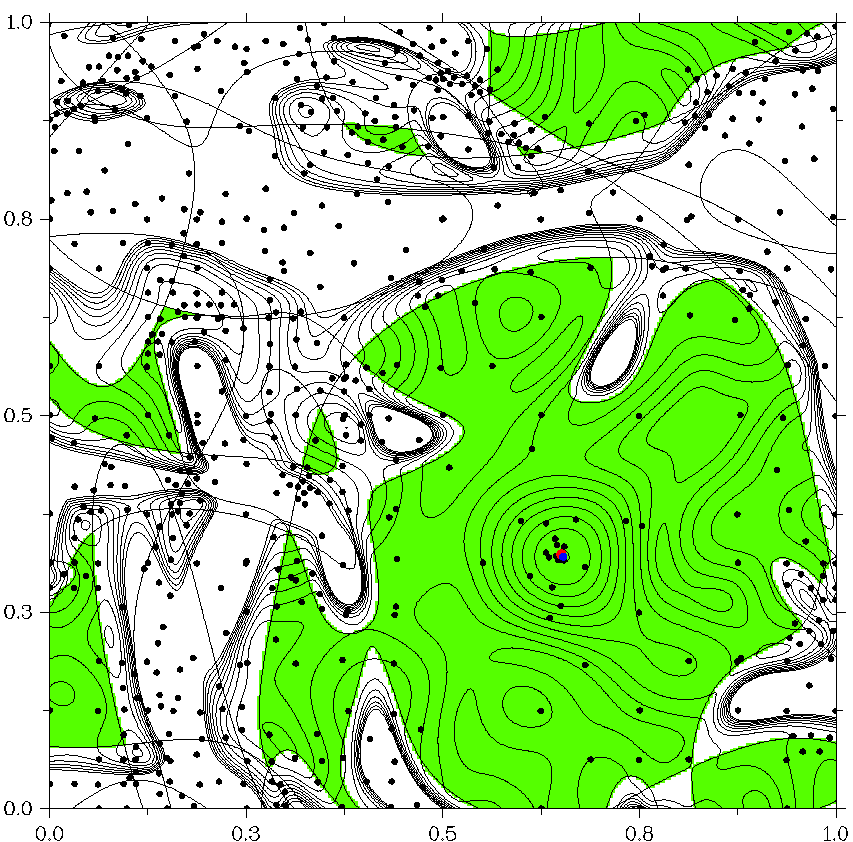
\includegraphics[width=1.0\linewidth]{vag_04.png} \\ (a)}
\end{minipage}
\hfill
\begin{minipage}{0.5\linewidth}
\center{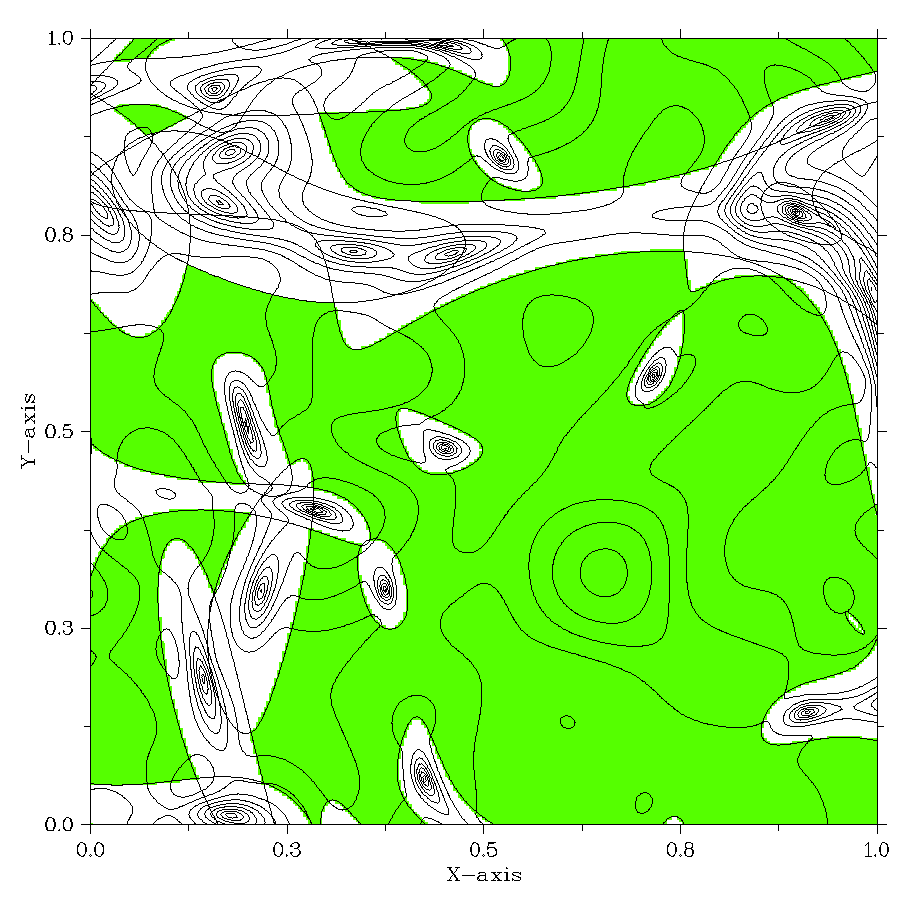
\includegraphics[width=1.0\linewidth]{vag_06.png} \\ (b)}
\end{minipage}
\caption{The problems based on functions (\ref{VAG}) }
\label{fig:VAG}
\end{figure}


\section {Conclusion}

This paper considers the method for generating global optimization test problems with non-convex constraints that allows:
\begin{itemize}
	\item to control the size of feasible domain with respect to the whole domain of the parameters' variation;
	\item to known a priori the conditional global minimizer of the objective function;
	\item to generate the unconditional global minimizer of the objective function out of the feasible domain (to simulate the constraints and objective function in the applied optimization problems).
\end{itemize}

The demonstration of the developed approach in application to well-known index method for solving complex multiextremal optimization problems with non-convex constraints is considered.

The developed approach allows generating any number of test global optimization problems with non-convex constraints for performing multiple computational experiments in order to obtain a reliable evaluation of the efficiency of the developed optimization algorithms.

% Acknowledgement
\section{ACKNOWLEDGMENTS}
This research was supported by the Russian Science Foundation, project No 16-11-10150.

% References

%\nocite{*}
\bibliographystyle{aipnum-cp}%
\bibliography{LeGo}%


\end{document}
